\documentclass[margin=3pt,
  convert,
  convert={
    outext=.png,
    command=\unexpanded{
      pdftocairo -r 300 -png \infile % 将生成的pdf文件转换为png图像
    }
  }
  ]{standalone}

\usepackage{tikz}
\usetikzlibrary{intersections, calc}

% 求两个路径交点
% #1 第1路径名称
% #2 第2路径名称
% #3 交点名称,同时定义了一个全局宏\InterNb记录了交点总数
\newcommand{\intersec}[3]{%
  \path[name intersections={of=#1 and #2, by=#3, sort by=#1,total=\t}]
  \pgfextra{\xdef\internb{\t}};
}

% 过指定点到曲线的垂线
% #1 路径名称
% #2 路径上指定点坐标
% #3 交点坐标
\newcommand{\insecvline}[3]{
  % 过#2点的垂线
  \path[name path = v](#2|-current bounding box.south) -- (#2|-current bounding box.north);  
   % 求路径#1与路径v的交战,并记为#3
  \intersec{#1}{v}{#3}

  \draw[red, dashed] (#2)--(#3);
  
}

  


\begin{document}
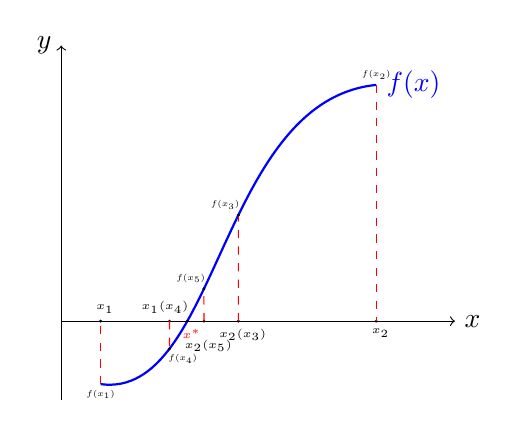
\begin{tikzpicture}[
  domain=1.5:4.1,
  samples=101,
  ]
  % 绘制命名曲线
  \draw[blue,thick, name path=graph](0.5,-0.8) coordinate (fx1) .. controls (2.0,-1) and
  (2,2.8) .. (4, 3) coordinate (fx2) node[right] {$f(x)$};
  % 绘制x轴和y轴
  \draw[->, name path=x] (0,0) -- (5,0) node[right] {$x$};
  \draw[->] (0,-1.0) -- (0,3.5) node[left] {$y$};

  % 绘制根的真值点
  \intersec{graph}{x}{x0}
  \fill[fill=black](x0) circle[radius = 0.02cm] node[red, scale = 0.8,
  below, shift={(2pt, 0pt)}, font=\tiny]{$x^*$};
  
  % 坐标定义
  \coordinate (x1) at (0.5, 0);
  \coordinate (x2) at (4.0, 0); 

  % 开始
  \fill[fill=black](x1) circle[radius = 0.02cm] node[black, scale = 0.8,
  above, shift={(2pt, 0pt)}, font=\tiny]{$x_{1}$};
  % 绘制垂线
  \draw[red, dashed] (fx1)node[black,scale = 0.6, below, shift={(0pt,0pt)}, font = \tiny] {$f(x_{1})$}--(x1);
  \fill[fill=black](x2) circle[radius = 0.02cm] node[black, scale = 0.8,
  below, shift={(2pt, 0pt)}, font=\tiny]{$x_{2}$};
  % 绘制垂线
  \draw[red, dashed] (fx2)node[black,scale = 0.6, above, shift={(0pt,0pt)}, font = \tiny] {$f(x_{2})$}--(x2);

  % 第1次迭代
  \coordinate (bx) at ($(x1)!0.5!(x2)$);
  \fill[fill=black](bx) circle[radius = 0.02cm] node[black, scale = 0.8,
  below, shift={(2pt, 0pt)}, font=\tiny]{$x_{2}(x_{3})$};
  \insecvline{graph}{bx}{fx} 

  \fill[fill=black](fx) circle[radius = 0.02cm] node[black, scale = 0.6,
  above, shift={(-8pt, 0pt)}, font=\tiny]{$f(x_{3})$};

  % 第2次迭代
  \coordinate (x2) at (bx);
  \coordinate (bx) at ($(x1)!0.5!(x2)$);
  \fill[fill=black](bx) circle[radius = 0.02cm] node[black, scale = 0.8,
  above, shift={(-2pt, 0pt)}, font=\tiny]{$x_{1}(x_{4})$};
  \insecvline{graph}{bx}{fx}

  \fill[fill=black](fx) circle[radius = 0.02cm] node[black, scale = 0.6,
  below, shift={(8pt, 0pt)}, font=\tiny]{$f(x_{4})$};
  
  % 第3次迭代
  \coordinate (x1) at (bx);
  \coordinate (bx) at ($(x1)!0.5!(x2)$);
  \fill[fill=black](bx) circle[radius = 0.02cm] node[black, scale = 0.8,
  below, shift={(2pt, -5pt)}, font=\tiny]{$x_{2}(x_{5})$};
  \insecvline{graph}{bx}{fx}
  
  \fill[fill=black](fx) circle[radius = 0.02cm] node[black, scale = 0.6,
  above, shift={(-8pt, 0pt)}, font=\tiny]{$f(x_{5})$};
  
  
  % % 绘制起始点
  % \fill[fill = black] (0.5, -0.8) coordinate (xs) circle[radius = 0.02cm] node[scale = 0.5, shift={(2pt, 0)},below, font = \tiny] {$x_{0}$};

  % % 通过循环绘制3次迭代结果
  % \foreach \X/\clr in {1/red, 2/green, 3/violet, 4/magenta}
  % {
  %   % 调整x轴点标记y方向偏移
  %   \ifodd\X
  %     \xdef\yoff{-3pt}
  %   \else
  %     \xdef\yoff{0pt}
  %   \fi
    
  %   % 过xs的垂线与曲线graph的交点
  %   \path[name path=v](xs|-current bounding box.south) -- (xs|-current bounding box.north);
  %   \intersec{graph}{v}{fx}
  %   \pgfmathsetmacro{\fxn}{int(\X-1)}
  %   \fill[fill = black] (fx) circle[radius = 0.02cm] node[scale = 0.6, left, shift={(2pt,3pt)}, font = \tiny] {$f(x_{\fxn})$};

  %   % 求切线端点
  %   \tanterms{graph}{fx}{li}{ri}
  %   % 定义切线路径,对得到的切线微元进行延长
  %   % 延长倍数和方向需要手动调整(需要改进)
  %   \path[name path=t](ri)--($(ri)!12!(li)$);
  %   \intersec{t}{x}{tx}
  %   \fill[fill = black] (tx) circle[radius = 0.02cm] node[scale = 0.5, shift={(2pt, \yoff)}, below, font = \tiny] {$x_{\X}$};
  %   % 绘制切线和垂线
  %   \draw[\clr, dashed] (fx)--(tx) (fx)--(xs);

  %   % 下一次迭代
  %   \coordinate (xs) at (tx);
  % }
\end{tikzpicture}
\end{document}

%%% Local Variables:
%%% mode: latex
%%% TeX-master: t
%%% End:
